\documentclass[a4paper,10pt]{article}
\usepackage[margin=15mm]{geometry}
\usepackage{pgf,tikz}
\usepackage{subfig}
\usepackage{amsmath}
\usepackage{color}
\usepackage{amssymb}
\usepackage{noweb}
\usepackage{listings}
\usetikzlibrary{circuits.logic.US}
\usetikzlibrary{positioning}
\usetikzlibrary{matrix}
 
\definecolor{dkgreen}{rgb}{0,0.6,0}
\definecolor{gray}{rgb}{0.5,0.5,0.5}
\definecolor{mauve}{rgb}{0.58,0,0.82}

\lstset{ %
  language=Verilog,                % the language of the code
  basicstyle=\footnotesize,           % the size of the fonts that are used for the code
  numbers=left,                   % where to put the line-numbers
  numberstyle=\tiny\color{gray},  % the style that is used for the line-numbers
  stepnumber=2,                   % the step between two line-numbers. If it's 1, each line 
                                  % will be numbered
  numbersep=5pt,                  % how far the line-numbers are from the code
  backgroundcolor=\color{white},      % choose the background color. You must add \usepackage{color}
  showspaces=false,               % show spaces adding particular underscores
  showstringspaces=false,         % underline spaces within strings
  showtabs=false,                 % show tabs within strings adding particular underscores
%  frame=single,                   % adds a frame around the code
  rulecolor=\color{black},        % if not set, the frame-color may be changed on line-breaks within not-black text (e.g. commens (green here))
  tabsize=2,                      % sets default tabsize to 2 spaces
  captionpos=b,                   % sets the caption-position to bottom
  breaklines=true,                % sets automatic line breaking
  breakatwhitespace=false,        % sets if automatic breaks should only happen at whitespace
  title=\lstname,                   % show the filename of files included with \lstinputlisting;
                                  % also try caption instead of title
  keywordstyle=\color{blue},          % keyword style
  commentstyle=\color{dkgreen},       % comment style
  stringstyle=\color{mauve},         % string literal style
  escapeinside={\%*}{*)},            % if you want to add LaTeX within your code
  morekeywords={*,...}               % if you want to add more keywords to the set
}
\usepackage{amsthm}
\usepackage{hyperref}
\setlength{\parskip}{3mm}
\newtheorem{axiom}{Axiom}
\newtheorem{definition}{Definition}
\newtheorem{comment}{Comment}
\newtheorem{example}{Example}
\newtheorem{lemma}{Lemma}
\newtheorem{prop}{Property}
\newtheorem{problem}{Problem}
\newtheorem{remark}{Remark}
\newtheorem{theorem}{Theorem}

% Title Page
\title{Introduction to VHDL}
\author{Dilawar Singh \footnote{His name is pronounced 'the law were'. He works in L.W.C.A. ( Lab Wihtout a Cool Acronym) and
can be contacted at \texttt{dilawar@ee.iitb.ac.in}}}
\date{\today}

\begin{document}
\maketitle

\begin{abstract}
  
  This is not a tutorial on but a brief introduction to VHDL language. It has
  been assumed that you have been using at least C/C++. 
  
  To do VHDL related assignments, you need not know full VHDL.  Only what 
  minimal is required discussed here. You need to know entity-architecture
  pair, data-types, and use of components in VHDL. And the best way to learn a
  language, mimicking Dodo the bird of \emph{Alice in Wonderland} one can say is
  to write some program in it. 

\end{abstract}

\section{Introduction}
  
 Let's begin with a toy shown in following figure. One exercise is immediate :
 \emph{Write its equivalent proto-RTL description}. Later, we can simply
 translate this proto-RTL description to VHDL (or any other HDL) by hand, or
 better, we can write a computer program to automate the conversion. This is
 what Mr. Sameer's (guide Prof. Madav Desai) AHIR tool-chain does : converts C
 programs to VHDL.

 In this document, we'll describe this circuit directly in VHDL.
 
  \begin{figure}[h] %% Dilawar Singh (c) 2012 - 2013
%% Circuit macros to produce amazing quality circuits
%% More amazing than powerpuff girls.
\def\mux { -- ++(0,-1) node [above right] {$1$} -- ++(0.6,0.2) -- 
++(0,0.6) -- ++(-0.6,0.2) -- cycle};
\def\muxr { -- node [below left] {$1$} ++(1,0) -- ++(-0.2,-0.6) -- 
++(-0.6,0) -- ++(-0.2,0.6)  -- cycle}

%% Multiplexor 
%% 3 params : location, size, name.  
%% Note : To connect wires
%% to north, east, south and west one should also use .center with name.

\newcommand{\multiplexer}[3]{
\draw #1 -- ++(0,-#2/4)  node (#3_input1) at ++(0,0) {\scriptsize{\hspace{8pt}1}}
-- ++(0,-#2/2) node (#3_input2) at ++(0,0){\scriptsize{\hspace{8pt}0}} 
-- ++(0,-#2/4) -- ++(#2/2,#2/4)
-- ++(0,#2/4) node(#3_output) [] {}  -- ++(0,#2/4) 
-- ++(-#2/4,#2/8) node(#3_select) {} -- ++(-#2/4,#2/8)
}

%% Register 
%% 4 parama : location, width, height, name 
%% Note : To connect wires to north, east, south and west one should 
%% also use .center with name.
\newcommand{\register}[4]{
\draw #1 -- ++(#2/2,0) node(#4_north){} --++(#2/2,0) 
% eastern side
-- ++(0,-#3/2) node(#4_east){} -- ++(0,-#3/2) 
% southern side 
-- ++(-#2/2,0) node(#4_south){} --++(-#2/2,0) 
% label 
-- ++(0,#3) node at ($#1+(#2/2+0.1,-#3/2)$) {#4} 
% the western triangle
-- ++(0.6*#3, -0.5*#3) -- ++(-0.6*#3, -0.5*#3)
% the western anchor
-- ++(0,#3/2) node (#4_west) {}
}

%% Bus
%% 3 params : from, to, size 
\newcommand*{\bus}[4] {
\draw[->] #1 -- #2 node[midway]{\tiny{/}} 
    node [#3] {\scriptsize{#4}}
}

%% D flip-flop
%% 4 params : left bottom, width, height, label
\newcommand{\dflipflop}[4] {
\draw #1 -- ++(#2/2,0) node(#4_set) at ++(0,0) [above] {\scriptsize{S}}
-- ++(#2/2,0) 
% qbar 
-- ++(0,#3/3) node (#4_qbar) at ++(0,0) [left] {\scriptsize{$\bar{Q}$}}
-- ++(0,#3*2/3)
% q
-- ++(0,#3/3) node (#4_q) at ++(0,0) [left] {\scriptsize{${Q}$}}
-- ++(0,#3/3)
% reset 
-- ++(-#2/2,0) node (#4_reset) at ++(0,0) [below] {\scriptsize{R}}
-- ++(-#2/2,0)
% D
-- ++(0,-#3/3) node (#4_d) at ++(0,0) [right] {\scriptsize{D}}
-- ++(0,-#3*2/3)
%% clock
-- ++(0, -0.2) -- ++(0.2,0.2) -- ++(-0.2, 0.2) -- ++(0, -0.2) 
node (#4_clock) at ++(0,0) [right]  {}
%% clock enable
-- ++(0,-#3/3) node (#4_ce) at ++(0,0) [right] {\scriptsize{CE}}
-- cycle
}

    \begin{center} \begin{tikzpicture}[circuit logic US]
        %\dflipflop{(c.center)}{2}{2}{``DFF''};
        %% Draw the combinational logic.
        \matrix[column sep=7mm] { \node (reset) {reset}; & & &  \\ \node (a)
        {a}; & \node[and gate] (a1) {}; &  &  \\ \node (b) {b};  & \node[not
        gate] (n1) {};& \node[or gate] (o1) {}; \\ \node (clk) {clk};  &  &  \\
        }; \node (dffNode) at ($(o1.east)+(1,-2)$) {};
        \dflipflop{(dffNode.center)}{1.5}{1.5}{dff}; \draw (reset) -|
        (dff_reset); \draw (a) -- ++(right:5mm) |- (a1.input 1); \draw (b) --
        ++(right:5mm) |- (a1.input 2); \draw (b) -- ++(right:5mm) |- (n1.input);
        \draw (n1.output) -| (o1.input 2); \draw (a1.output) -- ++(right:5mm) |-
        (o1.input 1); \draw (o1.output) -- ++(right:5mm) |- (dff_d); \draw (clk)
        -- ++(right:5mm) |- (dff_clock); \draw (dff_q) -- ++(right:10mm) node at
        ++(0,0) [above] {out}; \end{tikzpicture} \end{center}

    \caption{A small logic circuit. This represents one of the most commonly
    found hardware block : some combinational logic attached to the input of
    flip-flop.  We have D-type flip-flop on the right. Unused pins are
    \texttt{S} (set), $\bar{Q}$, and \texttt{CE} (clock-enable).}
 
    \label{fig:circuit}
 
  \end{figure}

\paragraph{}

  VHDL gives a block level abstraction of system. One needs to know the input and output
  (hereafter, \textbf{port}) of the system. We have \texttt{a}, \texttt{b},
  \texttt{clk}, and \texttt{reset} as input to (input port of) this system and
  \texttt{out} as the output (port) of this system shown in figure
  \ref{fig:circuit}. Immediately after this we ask the \textbf{type} of ports.
  We assume that all ports in this system have data-type \textbf{bit}
  \footnote{See the types available in VHDL language. VHDL type system is
  stronger than Verilog. Why should it matter?}.

  Till now, we have the following information about the system :

  \begin{table}[h] \centering \begin{tabular}{c|c|c} Port & Direction & Type \\
    \hline a & in & bit \\ b & in & bit \\ clk & in & bit \\ reset & in & bit \\
    out & out & bit \\ \hline \end{tabular} \end{table}


\section{Entity-Architecture pair in VHDL}
  
In VHDL, any digital system is described by \textbf{entity-architecture} pair.
\textbf{Entity} describes what a system receives as input nd what it generates
as output. \textbf{Architecture} describes how the system operates on input to
generate it's output. If an analogy is to be drawn with C/C++ languages, it can
be said that entity are like function declarations while architecture are like
function definitions. Enough philosophies! Let's see some code.

\lstinputlisting[language=vhdl, firstline=7 , caption=Entity declaration  ,
lastline=27]{../GHDLDemo/demo.vhd}

And now we have to write the \textbf{architecture} of this entity. There are two
style of writing architecture. One is called \textbf{structural} and other is
\textbf{behavioural}. If we already know the components (as we do for this
system) it is straightforward to write the structural description. When we do
not know the components and their arrangements (in most of the case we do not
know), we write behavioural description. 

\begin{remark}[Structral vs behaviour]
 
  Structural architecture describes \emph{what is connected with what}. In our
  system we have three gates connected with each other and their output is
  reflected to \texttt{out} at each rising edge of clock (D-flip flop will
  ensure that.). Behavioural architecture describes \emph{what happens when}
  which can be described by the following equation.

  \begin{equation} out = \begin{cases} (a \land b) \lor \neg b & \quad \text{on
    rising edge of clock and reset is unset}\\ \text{no change} &
    \text{otherwise} \end{cases} \end{equation} \end{remark}

\paragraph{Structural architecture} Now let's see how to write the structural
architecture.

  \lstinputlisting[language=vhdl , caption = We do not define the architecture
  of components used in this code.  Each component again has
  \textbf{entity-architecture} pair. We can write those in different files and
  compile that file separately using ghdl. How to do it is available in ghdl
  manual.  , firstline=27, lastline=74]{../GHDLDemo/demo.vhd}

  \paragraph{Behavioural architecture}

  This is a more natural way to describe the hardware. Most of the time we think
  in terms of behaviour of the circuit. 
 
  \lstinputlisting[language=vhdl , caption = Behavioural architecture ,
  firstline=75, lastline=200]{../GHDLDemo/demo.vhd}


  \begin{remark}{Multiple architecture}
    
    We can have any number of architectures for one entity. If we do so, it is
    not clear which which architecture to use with the entity. Standard practice
    in VHDL is to write \textbf{configuration}.
 
  \end{remark}

  \paragraph{Behavioural to hardware}
    
  Structural architecture is essentially a netlist of the circuit : which
  component is connected to which component. Therefore much is known about the
  circuit topology. But what about behavioural architecture? It is not always
  easy to convert a behavioural description to hardware despite the rising
  maturity of synthesis tools \footnote{Conversion of a description to a netlist
  of the hardware is called synthesis.} Fortunately for us, we are not concerned
  about synthesis in this course.  Anyway lets have a look at the hardware is
  generated by Xilinx tool.

  \begin{figure}[h] \centering
    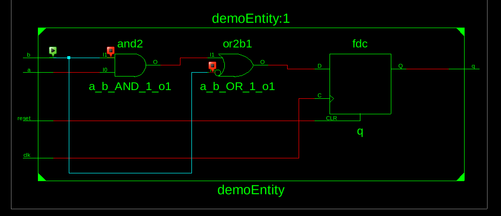
\includegraphics[width=\textwidth]{./../GHDLDemo/Xilinx/bhav.png}
    \caption{Hardware synthesised by Xilinx tool. Well, it looks like what we
    started with. In real life we usually do not know details of the hardware
    connections. Its bahaviour is specified and simulation is required to say
    something about its correctness. When we write code for simulation, we can
    full language. All constructs of a language are not supported by synthesise
    tool and one has to rewrite that particular section of code. A more recent
    language \textbf{bluespec} (available in HPC lab, IIT Bombay) guarantees
    that if you can compile it, you can synthesise it. } \label{fig:synthesis}

  \end{figure}

\end{document}          
